%
%  Appendix : Analysis
% =====================
%

\chapter{Simulation Analysis}
\label{Apx:SA}

This appendix details some of the key calculations used when analysing simulation data used for this thesis work.

% ================================================================================================================================ %
\section{Emittance and Twiss Parameters}
\label{Apx:SA:EnTwiss}

The Twiss parameters are useful quantities to describe the trajectory of particles in an accelerator in the transverse phase space.
The following, brief, derivation is based on Klauss Wille, \textit{The Physics of Particle Accelerators}~\cite{wille:2001}.

The general solution to the trajectory of particles in an accelerator is given by
\begin{align}
    x(s)          &=  \sqrt{\epsilon\beta(s)} \cos\left[\Psi(s) + \phi\right] \label{EQ:PTrajX} \\
    x^{\prime}(s) &= -\sqrt{\frac{\epsilon}{\beta(s)}}
                     \left[\alpha(s)\cos\left(\Psi(s) + \phi\right) + \sin\left(\Psi(s) + \phi\right)\right], \label{EQ:PTrajXP}
\end{align}
where the parameter
\begin{equation}
    \alpha(s) \equiv -\frac{\beta^{\prime}(s)}{2}. \label{EQ:TwissAlpha}
\end{equation}

In order to arrive at an expression describing the particle motion in the $x$--$x^\prime$ plane, we must eliminate the terms depending on $\Psi$.
We thus obtain:
\begin{equation}
    \epsilon = \frac{x^2}{\beta(s)} + \left(\frac{\alpha(s)}{\sqrt{\beta(s)}}x + \sqrt{\beta(s)}x^{\prime}\right)^2.
\end{equation}

By introducing the parameter
\begin{equation}
    \gamma(s) \equiv \frac{1+\alpha^2(s)}{\beta(s)}, \label{EQ:TwissGamma}
\end{equation}
we obtain
\begin{equation}
    \epsilon^2 = \gamma(s)x^2(s) + 2\alpha(s)x(s)x^{\prime}(s) + \beta(s)x^{\prime 2}(s). \label{EQ:EmittFull}
\end{equation}

This equation describes an ellipse in phase space, and how the Twiss parameters $\alpha$, $\beta$ and $\gamma$ relates to the geometric emittance $\epsilon$ and the shape of the ellipse is illustrated in Figure~\ref{Fig:Twiss}.

\begin{figure}[hbt]
    \centering
    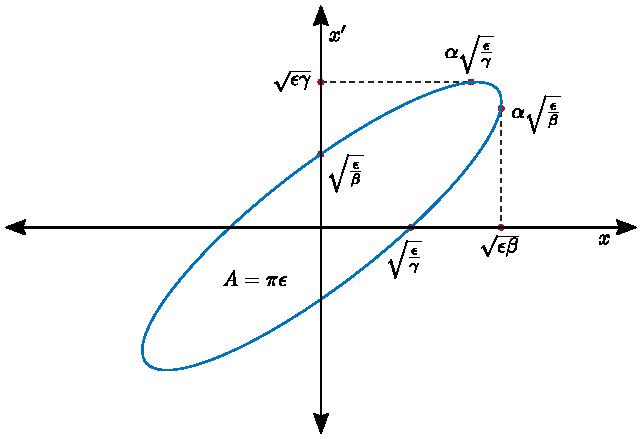
\includegraphics[width=0.8\linewidth,trim={0mm 0mm 0mm 0mm},clip]{figures/Twiss}
    \caption{\label{Fig:Twiss} The phase space ellipse of bunch particles. The figure is recreated from Figure 3.23 by Klauss Wille in \textit{The Physics of Particle Accelerators}~\cite{wille:2001}.}
\end{figure}

% ================================================================================================================================ %
\subsection{Extracting Twiss Parameters from Simulation Data}
\label{Apx:SA:EnTwiss:Sim}

Both OSIRIS and QuickPIC dump the macro particles as large arrays of six-dimensional data, providing each particle's position and momentum vector.
To study the collective motion of particles, it is useful to calculate the bunch total emittance in terms of the RMS value or standard deviation of its particles.
Equation~\ref{EQ:EmittFull} can be rewritten in terms of the statistical distributions of its particles such that
\begin{equation}
    \epsilon = \sqrt{\gamma\sigma_{x}^{2} + 2\alpha\sigma_{x}\sigma_{x^{\prime}} + \beta\sigma_{x^{\prime}}^{2}}, \label{EQ:Emitt}
\end{equation}
where the angle of the $i$-th particles can be taken from its momentum
\begin{equation}
    x_{i}^{\prime} = \frac{p_{i,x}}{p_{i,z}}.
\end{equation}

For a set of macro particles, the emittance can be calculated directly by taking the covariance matrix of the $x$ and $x^{\prime}$ vectors
\begin{equation}
    \mathbf{T} = \mathrm{cov}\left(\mathbf{x}, \mathbf{x}^{\prime}\right), \label{EQ:ECalc1}
\end{equation}
and then taking the square root of its determinant
\begin{equation}
    \epsilon = \sqrt{\mathrm{det}\left(\mathbf{T}\right)}. \label{EQ:ECalc2}
\end{equation}
The Twiss parameters can be extracted from the matrix $\mathbf{T}$ as well:
\begin{equation}
    \alpha = \mathrm{T}_{12}/\epsilon, \quad
    \beta  = \mathrm{T}_{11}/\epsilon, \quad
    \gamma = \mathrm{T}_{22}/\epsilon
\end{equation}

% ================================================================================================================================ %
\section{A Measure for Beam Quality}
\label{Apx:SA:QTilde}

For the emittance study in Publication~\ref{Pub:BL17}, it was necessary to define a convenient unit for the quality of the accelerated bunch in terms of emittance evolution in regions along the bunch length.
In the quasi-linear plus non-linear regime this publication investigates, emittance growth only occurs at the head of the bunch.
However, the region of emittance growth varies when parameters such as charge and beam size changes.
In the study, we defines the quantity
\begin{equation}
    \tilde{Q} = \sum_{m=0}^{M} \frac{1}{N} \left[\sum_{n=0}^{N} Q_{m+n}\right] \cdot \chi(\xi_{m},N),
\end{equation}
where $M$ is the number of longitudinal grid slices of length $\Delta\xi$ which contains macro particles for the witness bunch, and with corresponding coordinate $\xi_{m}$; $N$ is the number of such slices to average over; and $\chi(\xi_{m},N)$ is the step function
\begin{equation}
    \chi(\zeta,N) =
    \begin{cases}
        0, & \frac{\epsilon(\zeta) - \epsilon_{0}}{\epsilon_{0}} > 5\% \\
        1, & \frac{\epsilon(\zeta) - \epsilon_{0}}{\epsilon_{0}} \leq 5\%
    \end{cases}
    \quad\mathrm{for}\quad
    \xi_{m} < \zeta \leq \xi_{m} + N\Delta\xi,
\end{equation}
where $\epsilon(\zeta)$ is the emittance as defined by Equations~\ref{EQ:ECalc1} and~\ref{EQ:ECalc2} for a set of macro particles within the interval $\xi_{m}$ to $\xi_{m} + N\Delta\xi$.
For the studies included in Publication~\ref{Pub:BL17},
\begin{equation}
    M = \left\lfloor \frac{10\sigma_{z}}{\Delta\xi} \right\rceil, \quad
    N = 4.
\end{equation}
The first slice
\begin{equation}
    \xi_{0} = \mu_{\mathrm{eb}} - 5\sigma_{z,\mathrm{eb}} - 0.5\Delta\xi,
\end{equation}
where $\mu_{\mathrm{eb}}$ is the longitudinal centre of the bunch.

\paragraph{Note:} This method may yield a misleading result if the Twiss parameter $\alpha$ varies too much along the length of the bunch.
That is, the emittance can be locally small, and qualify for the $5\%$ criterion, even if the total emittance of the region included in $\tilde{Q}$ is not.
This can easily be checked after the seemingly optimal region of the bunch is known by verifying that its total emittance does not exceed the same criterion.

% ================================================================================================================================ %
